\documentclass{article}
\usepackage{graphicx} % Required for inserting images
\usepackage{float}

\title{Sistemi Operativi}
\author{Tommaso Trentin, Leonardo Ciscato Pajello}
\date{June 2025}

\begin{document}

\newpage
\tableofcontents
\newpage
\section{Definizione Machine Learning}
Campo di studio che da a computer abilità di imparare senza programmazione esplicita.\\
Si dice che un programma impara da un'esperienza E rispetto a task T e misurazioni di performance P se la sua performance su T, misurata con P, migliora con esperienza E.
Gli algoritmi di ML si dividono in:
\begin{itemize}
    \item Supervised learning
    \item Unsupervised learning
    \item Reinforcement learning
\end{itemize}
\section{Supervised Learning}
\begin{itemize}
    \item \textbf{Classificazione}: un algoritmo cerca di stimare \textit{decision boundary}
     (linea che separa dati)
    \begin{figure} [H]
        \centering
        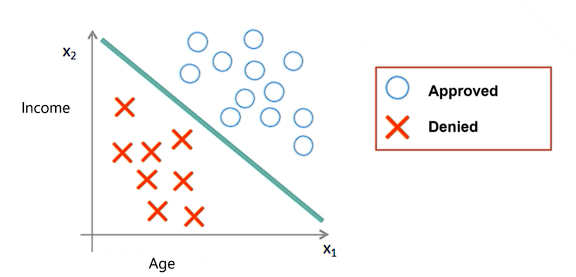
\includegraphics[width=0.7\linewidth]{img/image.png}
    \end{figure}
    \item \textbf{Concetto chiave $\#$1}: ogni oggetto rappresentato con set di numeri che ne rappresentano gli attributi (oggetti mappabili in 2D)
    \item \textbf{Concetto chiave $\#$2}: se ho più attributi aggiungo numeri al set per ogni attributo (oggetti mappabili in 3D+)
\end{itemize}
\subsection{Regressione}
Ha come abbiettivo la stima di valori, la stima può avvenire mediante retta di regressione lineare o logaritmica:
\begin{figure}[H]
    \centering
    \begin{minipage}[b]{0.48\textwidth}
        \centering
        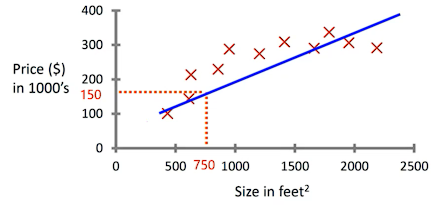
\includegraphics[width=0.85\textwidth]{img/intro_reg_lin.png}
        \caption{Regressione lineare}
    \end{minipage}
    \hfill
    \begin{minipage}[b]{0.48\textwidth}
        \centering
        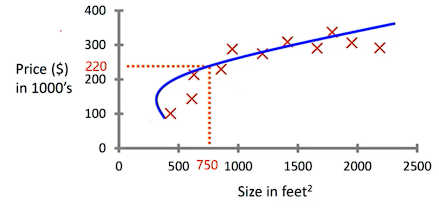
\includegraphics[width=0.85\textwidth]{img/intro_reg_log.png}
        \caption{Regressione logaritmica}
    \end{minipage}
\end{figure}
Una volta determinata la retta di regressione, dato uno dei due valori si può effettuare la stima dell'altro
\begin{figure} [H]
    \centering
    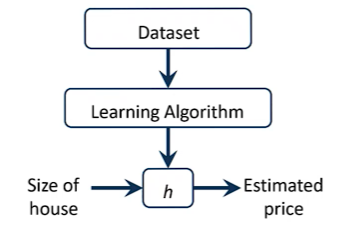
\includegraphics[width=0.5\linewidth]{img/stima.png}
    \caption{h = hypothesis}
\end{figure}
\end{document}
